% Use only LaTeX2e, calling the article.cls class and 12-point type.

\documentclass[12pt]{article}

% Users of the {thebibliography} environment or BibTeX should use the
% scicite.sty package, downloadable from *Science* at
% http://www.sciencemag.org/authors/preparing-manuscripts-using-latex 
% This package should properly format in-text
% reference calls and reference-list numbers.

\usepackage{scicite}

\usepackage{times}

%ONES I ADDED
\usepackage{graphicx} %Package for adding figures
\usepackage{authblk}
\usepackage{url} % for easy url hyperlinks
\usepackage{amsmath,amssymb}


\DeclareMathOperator{\E}{\mathbb{E}}

% The preamble here sets up a lot of new/revised commands and
% environments.  It's annoying, but please do *not* try to strip these
% out into a separate .sty file (which could lead to the loss of some
% information when we convert the file to other formats).  Instead, keep
% them in the preamble of your main LaTeX source file.


% The following parameters seem to provide a reasonable page setup.

\topmargin 0.0cm
\oddsidemargin 0.2cm
\textwidth 16cm 
\textheight 21cm
\footskip 1.0cm


%The next command sets up an environment for the abstract to your paper.

\newenvironment{sciabstract}{%
\begin{quote} \bf}
{\end{quote}}


% Include your paper's title here

\title{The search behaviour of terrestrial mammals}


% Place the author information here.  Please hand-code the contact
% information and notecalls; do *not* use \footnote commands.  Let the
% author contact information appear immediately below the author names
% as shown.  We would also prefer that you don't change the type-size
% settings shown here.

\author[1]{Michael J. Noonan$^\ast$}
\affil[1]{\small The University of British Columbia Okanagan, Kelowna, BC, Canada}

\author[2]{Ricardo Martinez-Garcia}
\affil[2]{\small ICTP South American Institute for Fundamental Research \& Instituto de Física Teórica, Universidade Estadual Paulista - UNESP, Rua Dr. Bento Teobaldo Ferraz 271, Bloco 2 - Barra Funda, 01140-070 São Paulo, SP, Brazil}

\author[3,4]{C. H. Fleming}
\affil[3]{Department of Biology, University of Maryland, College Park, MD, USA}
\affil[4]{\small Smithsonian Conservation Biology Institute, Front Royal, VA, USA}

\author[2]{Benjamin Garcia De Figueiredo}

\author[]{DATA PROVIDERS}

\author[3]{William F. Fagan}

\author[5,6,3]{Justin M. Calabrese}
\affil[5]{Center for Advanced Systems Understanding (CASUS), Görlitz, Germany}
\affil[6]{Helmholtz-Zentrum Dresden-Rossendorf (HZDR), Dresden, Germany}


%\author
%{Michael J. Noonan,$^{1\ast}$, Ricardo Martinez-Garcia,$^{2 \ast}$ Christen H. Fleming,$^{1,2}$, DATA PROVIDERS, Justin M. Calabrese$^{1,2}$\\
%\\
%\normalsize{$^{1}$The University of British Columbia Okanagan, Kelowna, BC, Canada}\\
%\normalsize{$^{2}$Smithsonian Conservation Biology Institute, National Zoological Park,}\\
%\normalsize{$^{3}$Smithsonian Conservation Biology Institute, National Zoological Park,}\\
%\normalsize{1500 Remount Rd., Front Royal, VA 22630, USA}\\
%\normalsize{$^{4}$Department of Biology, University of Maryland, College Park, MD 20742, USA}\\
%\\
%\normalsize{$^\ast$To whom correspondence should be addressed; E-mail:  michael.noonan@ubc.ca.}
%}

% Include the date command, but leave its argument blank.

\date{}



%%%%%%%%%%%%%%%%% END OF PREAMBLE %%%%%%%%%%%%%%%%



\begin{document} 

% Double-space the manuscript.

\baselineskip24pt

% Make the title.

\maketitle 



% Place your abstract within the special {sciabstract} environment.

\begin{sciabstract}
Animals searching landscapes need to strike a balance between finding sufficient resources, while also minimizing encounter with predators. A key determinant of encounter rates is the average length scale over which ballistic motion is maintained, with ballistic movement leading to higher encounter rates than more diffusive movement. Using GPS data from 53 species, we show how the optimization of search strategies underpins broad patterns in the movement terrestrial mammals. Ballistic length scales increase with body size, but predators maintained $\sim$250m longer ballistic length scales than similarly sized prey. These patterns emerge from a combination of bottom-up and top-down pressures, with individual deviations from the body-mass predictions being modulated by resource abundance. Our findings highlight the importance of encounter rates as a primary driver of mammalian movement.%The abstract should be 125 words or less.
\end{sciabstract}



% In setting up this template for *Science* papers, we've used both
% the \section* command and the \paragraph* command for topical
% divisions.  Which you use will of course depend on the type of paper
% you're writing.  Review Articles tend to have displayed headings, for
% which \section* is more appropriate; Research Articles, when they have
% formal topical divisions at all, tend to signal them with bold text
% that runs into the paragraph, for which \paragraph* is the right
% choice.  Either way, use the asterisk (*) modifier, as shown, to
% suppress numbering.

%\section*{Introduction}


\noindent As motile organisms move through landscapes in search of food and mates, they need to strike a balance between finding sufficient resources to grow and reproduce, while also minimizing the rate at which they encounter predators \cite{Milinski:1978,Visser:2006}. Because of the fitness consequences of foraging success \cite{Charnov:1976wz, Lemon:1991} and predator-prey dynamics \cite{Volterra:1928,May:1972,Fryxell:2007}, there should be strong selection pressure on movement strategies that optimize encounter rates. Although the exact movement processes that searching animals might take has been debated \cite{Viswanathan:1999,Edwards:2007,Sims:2008,Martinez:2020}, the general consensus is that ballistic (i.e., directed) movement leads to higher encounter rates than more diffusive (i.e., tortuous) movement \cite{Viswanathan:1999,Visser:2006,Edwards:2007,Hutchinson:2007,Bartumeus:2008,Sims:2008}. This occurs because individuals that exhibit diffusive movement will tend to repeatedly search over the same areas, whereas ballistic motion allows individuals to search over a larger area within the same amount of time. The average length scale over which ballistic motion is maintained, $l_v$ (in m), is thus a key determinant of encounter rates \cite{Visser:2006, Tejedor:2012} and a potent trait on which natural selection may act.

Because ballistic movement is the more efficient search strategy, bottom-up pressure exerted by food needs will select for longer ballistic length scales. Importantly, however, increasing $l_v$ will also increase the rate at which individuals encounter predators \cite{Milinski:1978,Visser:2006}. Top-down predation pressure thus selects for shorter ballistic length scales. Prey species searching for immobile vegetation must therefore optimize their movement against the opposing forces of their energetic requirements selecting for longer $l_v$, and predation pressure selecting for shorter $l_v$ \cite{Visser:2006}. Predatory species, in contrast, also benefit from maintaining longer ballistic length scales \cite{Visser:2006}, but without the top-down predation pressure experienced by prey species. The combination of bottom-up and top-down regulation is thus expected to select for longer ballistic length scales in predators, versus relatively more diffusive movement in prey species, all else being equal \cite{Visser:2006} (Fig.~\ref{fig:theory}). 

\begin{figure}[!h]
\centering
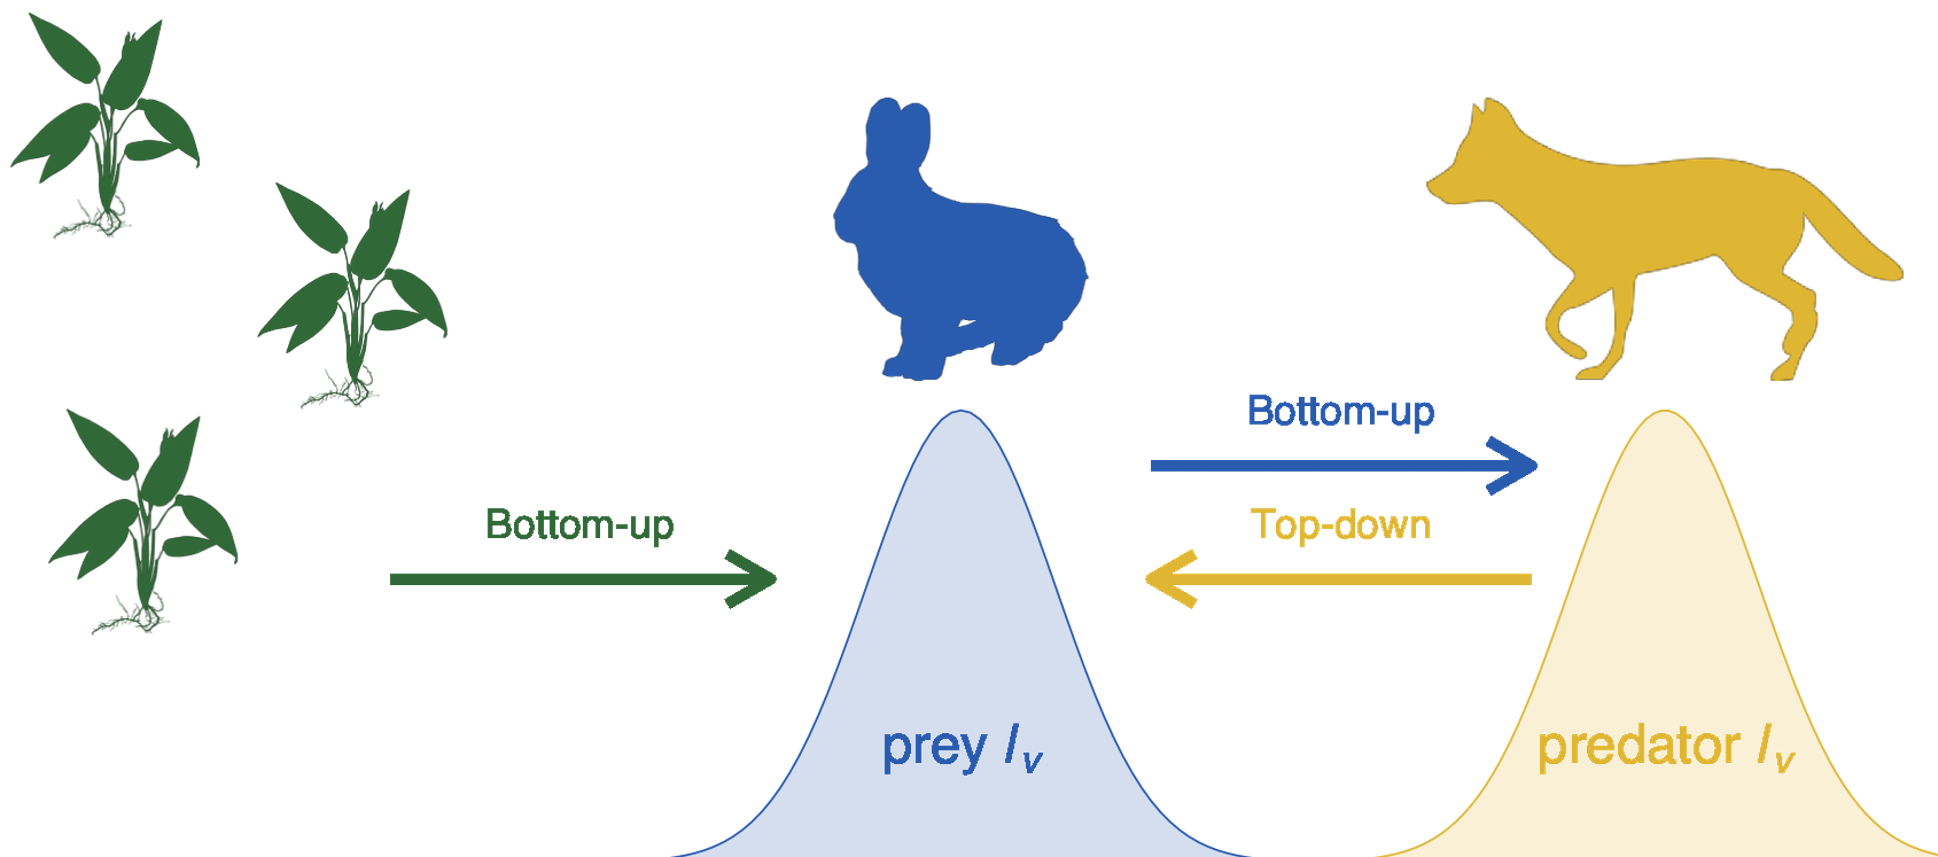
\includegraphics[scale=1]{Diagram_V2.png}
\caption{\textbf{Selection pressures on predator and prey ballistic length scales.} Schematic representation of bottom-up energetic requirements selecting for longer $l_v$, and top-down predation pressure selecting for shorter $l_v$.}
\label{fig:theory}
\end{figure}

Notably, `all else' is rarely equal in ecological systems, and the relative importance of bottom-up versus top-down regulation is highly context specific. In resource poor ecosystems, individuals need to spend a significant amount of time searching for food \cite{White:1978,Viswanathan:1999,Paiva:2010}. Because starvation is often a greater source of mortality than predation \cite{Mduma:1999}, the bottom-up driven need to find sufficient resources to survive should outweigh top-down pressure when resources are scarce. In productive environments, in contrast, bottom-up pressure on resource acquisition rates should be relaxed \cite{Charnov:1976wz,Viswanathan:1999,Dickie:2022}, allowing individuals to respond more directly to top-down pressure and maintain relatively more diffusive movement. These considerations lead to the expectation of a negative relationship between $l_v$ and environmental productivity.

Although the importance of $l_v$ in governing encounter rates is well recognised from a theoretical standpoint \cite{Bartumeus:2002,Visser:2006,Bartumeus:2008,Tejedor:2012}, a generalized understanding of how bottom-up (i.e., resource availability) and top-down (predation pressure) factors shape general patterns in mammalian search strategies is lacking. The primary reason for this is that movement data have, historically, been sampled at too coarse of a resolution to quantify the average length scale over which ballistic motion is maintained for a broad range of species \cite{Kays:2015en}. To see this, consider that $l_v$ is a function of the spatial variance of an animal's movement process ($\sigma_p$, in m$^2$, proportional to the home-range area) and its positional and velocity autocorrelation timescales ($\tau_p$ and $\tau_v$ respectively, in sec), given by
\begin{equation}
l_v = \sqrt{\frac{\tau_v}{\tau_p}\sigma_p}.
\label{eq:lv}
\end{equation}
While $\sigma_p$ can be well estimated from coarse data \cite{AKDEvsKDE}, autocorrelation structures are only revealed when the time scale of measurement is less than or equal to the autocorrelation timescales \cite{Noonan:2019}. In particular, $\tau_v$ tends to be on the order of minutes to hours for terrestrial mammals \cite{Morato:2016ioa,Noonan:2019,Medici:2022}. %As a result, ballistic length scales have only been explored in a small number of bacterial and planktonic species \cite{Visser:2006}.

Here, we leverage the rapid advances in the field of movement ecology \cite{Kays:2015en, Nathan:2022} that have enabled $l_v$ to be estimated for a broad range of species. We annotated Global Positioning System (GPS) location data on 963 individuals from 53 species of terrestrial mammals (Fig.~\ref{fig:emp_res}A) with mean adult body size (ranging from 0.4 to 4,000 kg), trophic group (herbivorous/frugivorous {\it n = 33}, and carnivorous {\it n = 20}). We restricted our analyses to range-resident animals and used continuous-time stochastic processes \cite{Calabrese:2016ey} to estimate $l_v$ for each individual (Fig.~\ref{fig:emp_res}B). We also annotated each data point with the mean Normalized Difference Vegetation Index (NDVI), a satellite-derived measure of resource abundance \cite{Pettorelli:2011}, to which each individual was exposed. %Finally, we quantified the mean percent forest cover \cite{Tuanmu:2014} at each sampled location as a measure of habitat permeability.

\begin{figure}[!h]
\centering
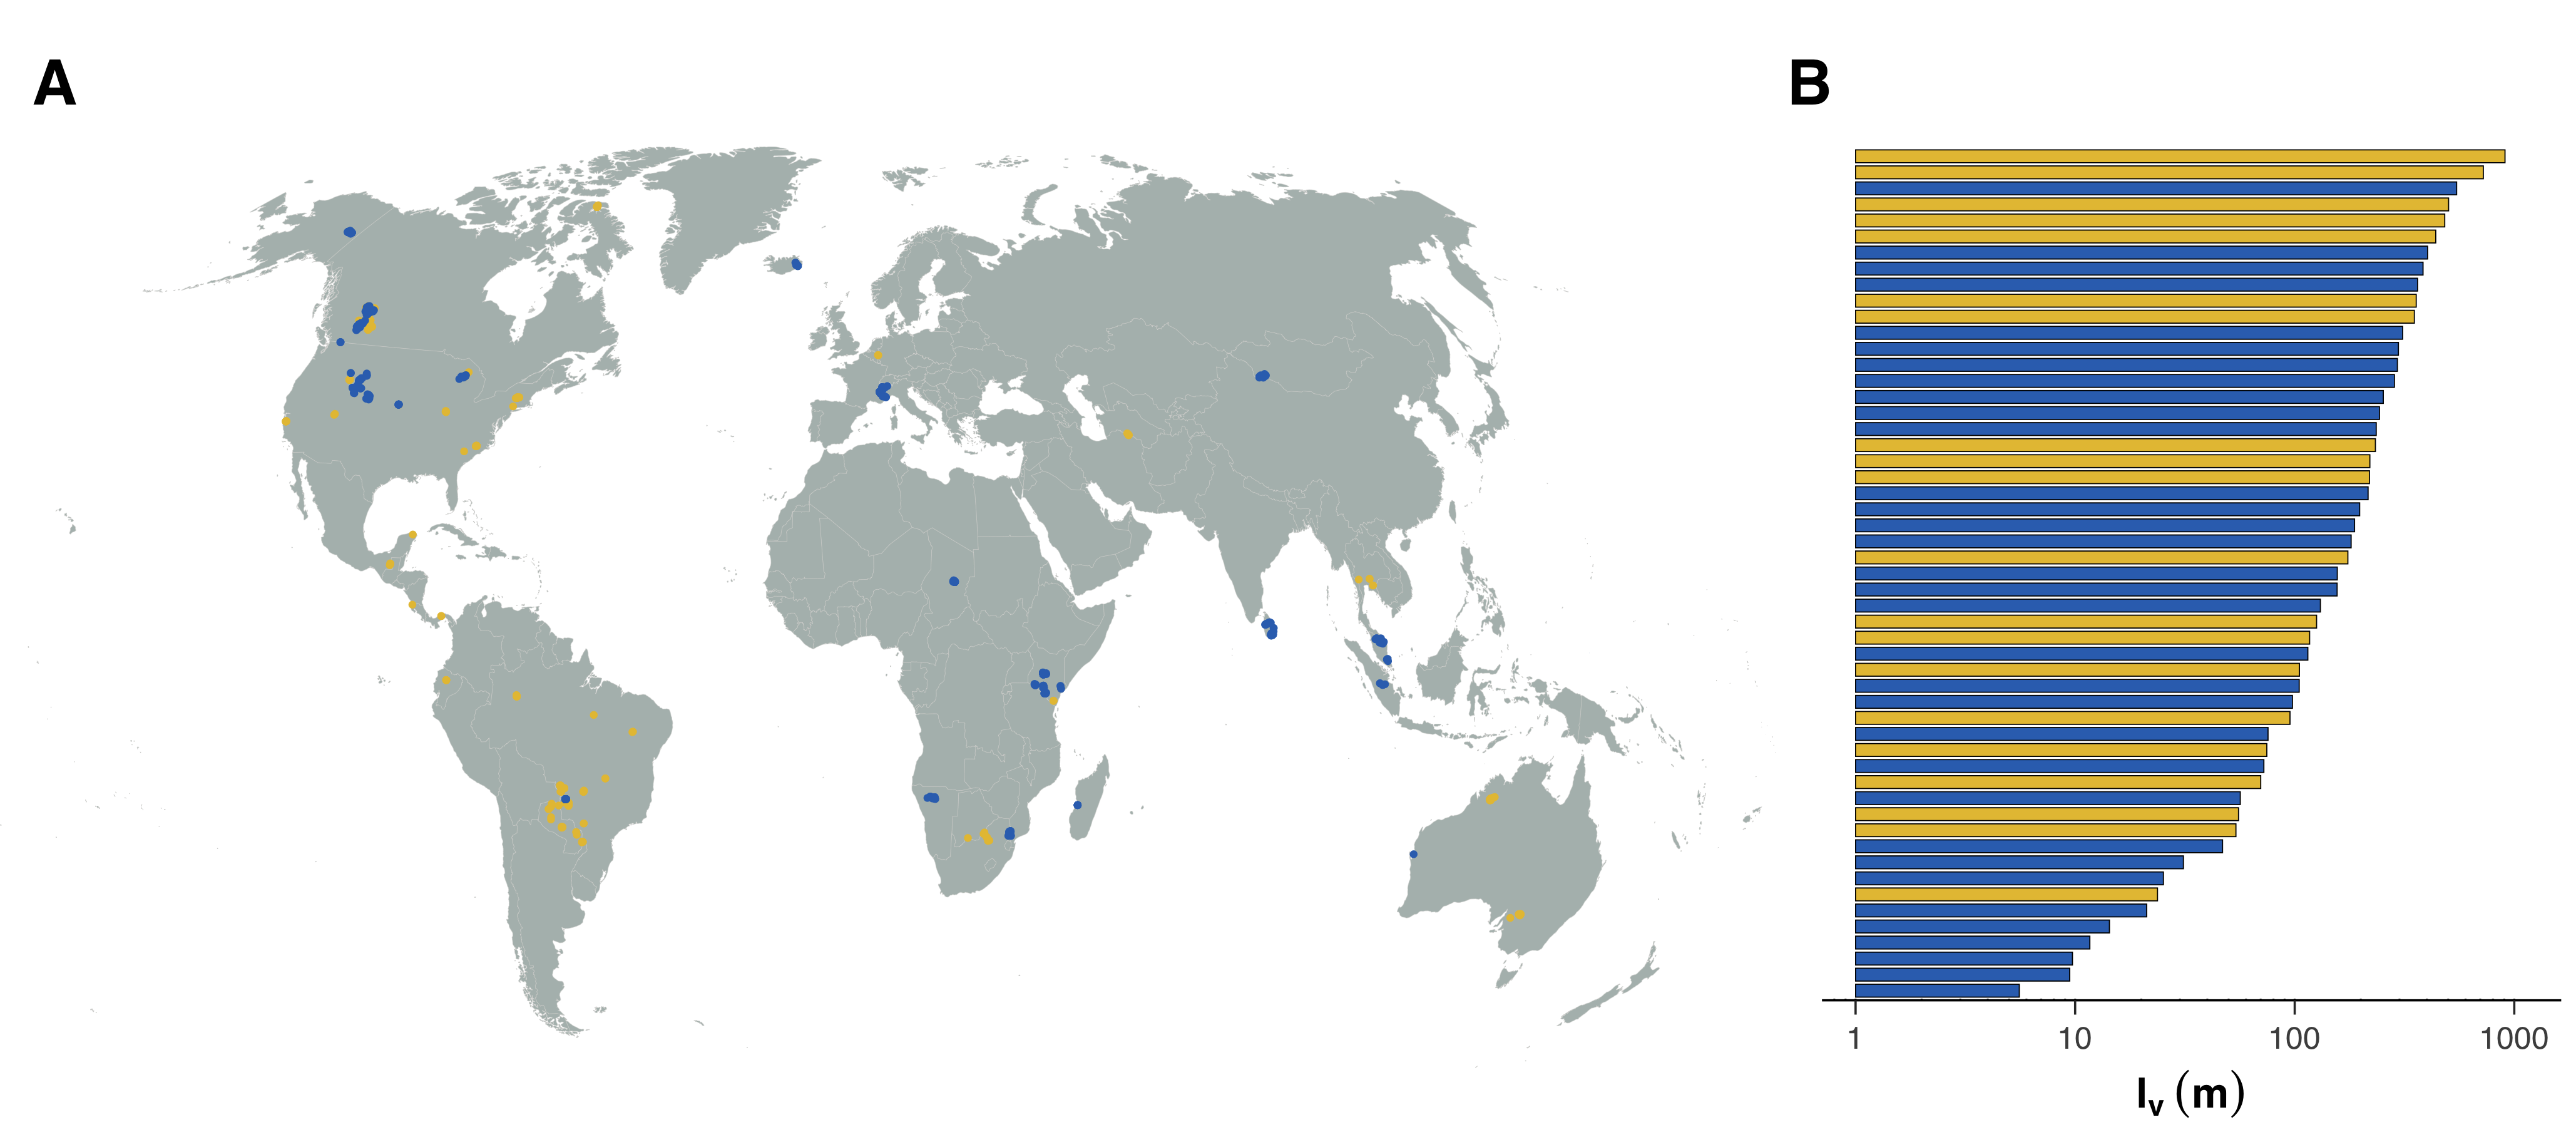
\includegraphics[scale=0.9]{Map.png}
\caption{\textbf{The distribution of mammalian movement data.} In A, the GPS locations of 963 prey (blue) and predatory (yellow) mammals across 53 species are plotted on the global map; and B shows the median ballistic length scales, $l_v$, for each species.}
\label{fig:map}
\end{figure}


These analyses revealed allometric scaling in both predator and prey ballistic length scales, with larger mammals tending to have longer $l_v$, all else being equal (Fig.~\ref{fig:emp_res}A). The body mass residuals followed theoretical predictions, with predator $l_v$ being approximately 260m longer than that of comparably sized prey species (Fig.~\ref{fig:emp_res}B). Least-squares regression also revealed a strong negative correlation between NDVI and the residuals of the allometric relationships in $l_v$ for predators and prey (Fig.~\ref{fig:emp_res}D). This was favoured over the null model of no relationship with NDVI by a $\Delta$AIC\textsubscript{c} of $>50$ for predators and a $\Delta$AIC\textsubscript{c} of $\sim900$ for prey. In other words, when resource abundance was ignored, predictions from the simple body-size relationships tended to underestimate observed $l_v$ in low-productivity ecosystems, and over-estimate $l_v$ in highly productive ecosystems. That bottom-up pressures appear to outweigh top-down pressure in resource scarce ecosystems is made all the more poignant when contrasted against patterns in trophic structure scaling. Resource poor environments tend to be more top heavy than productive ecosystems \cite{Hatton:2015}, effectively increasing individual level predation pressure.

\begin{figure}[!h]
\centering
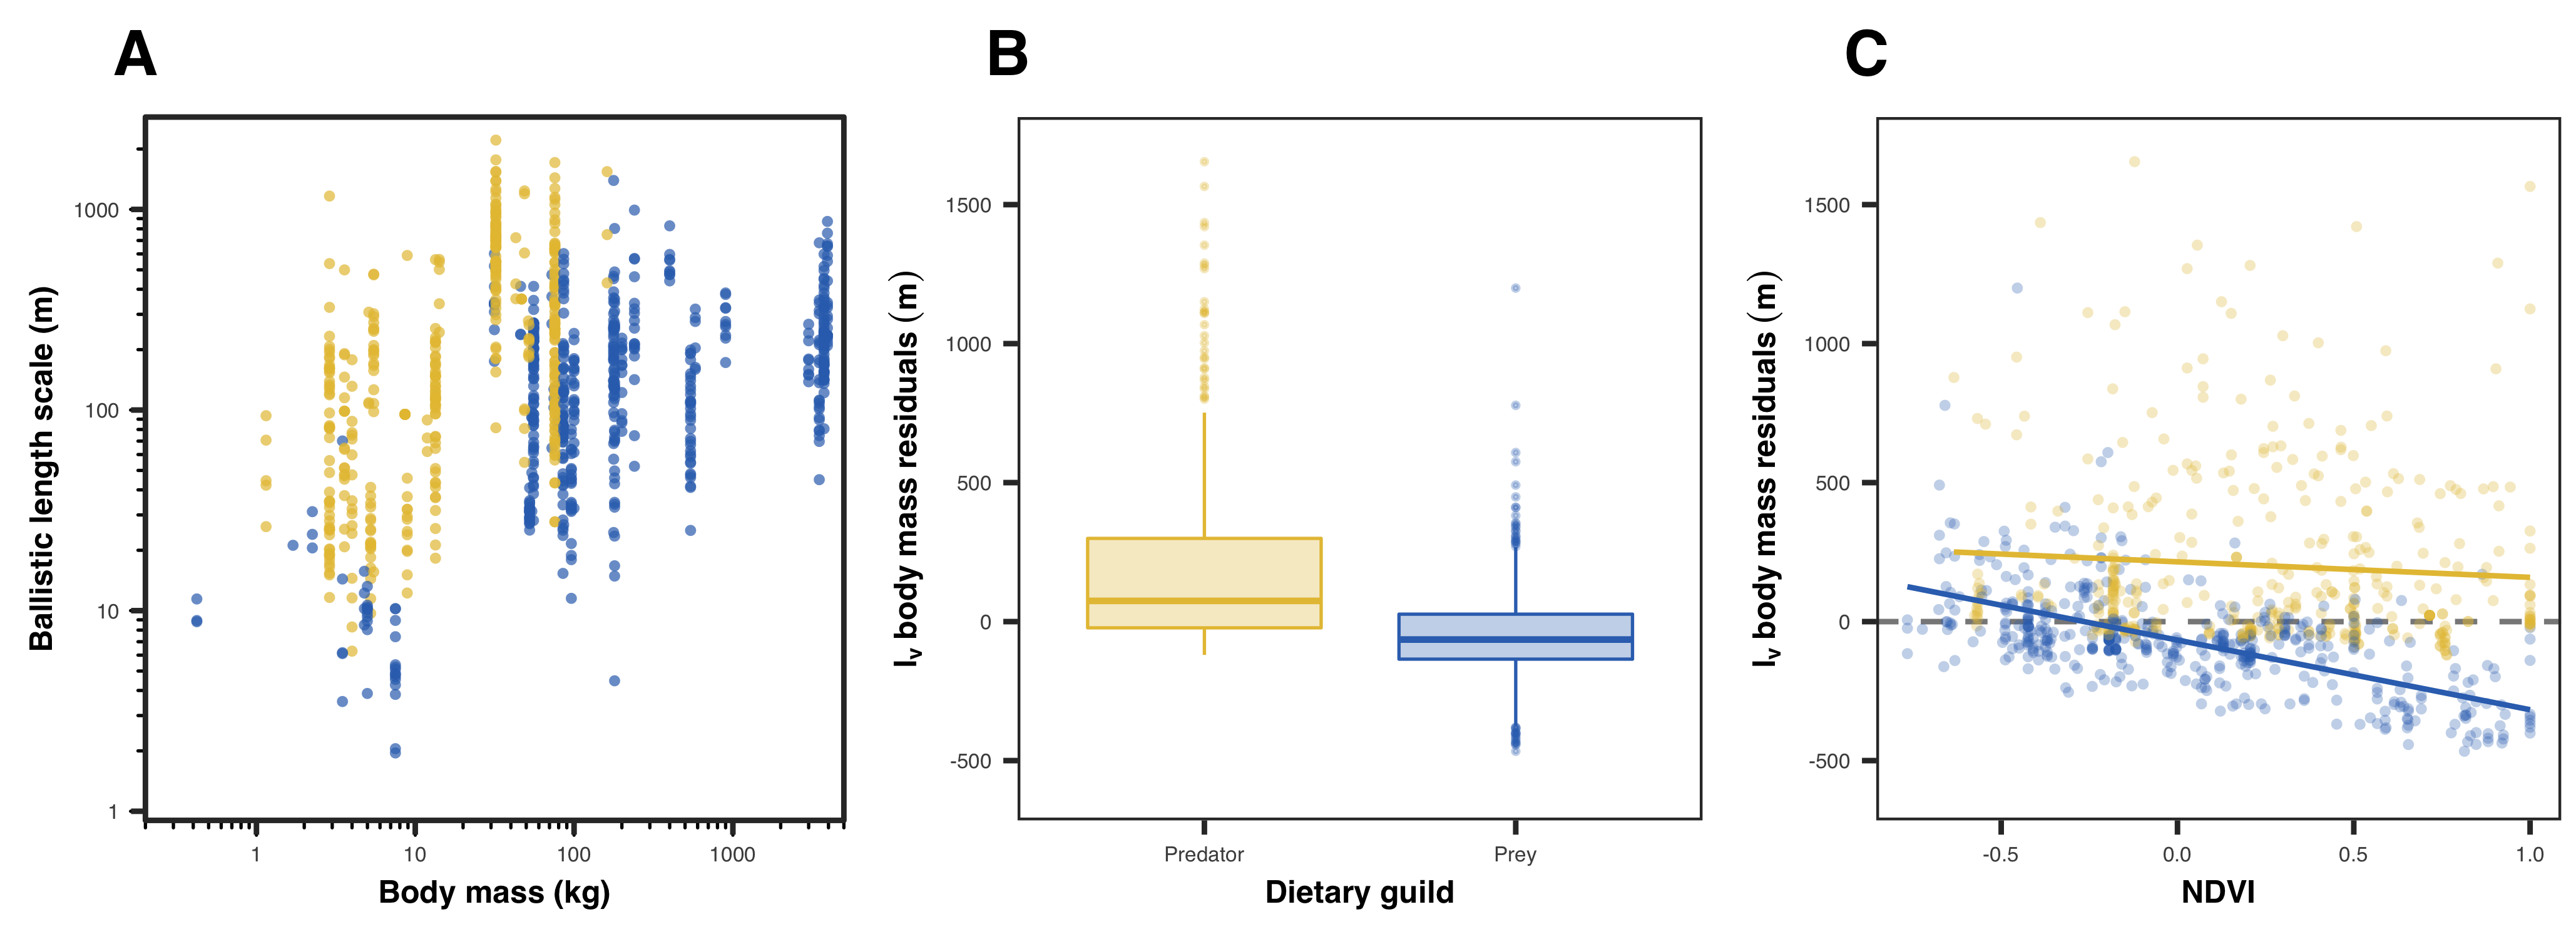
\includegraphics[scale=0.9]{Empirical_Trends.png}
\caption{\textbf{Trends in mammalian ballistic length scales.} Mammalian $l_v$ scales with body size, but predators exhibit more ballistic motion than prey species, and search behaviour is modulated by environmental productivity. The scatterplot in (\textbf{A}) show the allometric scaling of the ballistic length scale, $l_v$ for prey (blue), as well as predatory (yellow) mammals. The boxplots in (\textbf{B}) show the residuals of the body mass scaling of $l_v$ for predators and prey. When body size is accounted for, predatory species have significantly longer ballistic length scales on average ($P$ value $<10^{-15}$). The scatterplot in (\textbf{C}) show the body mass residuals as a function of the normalized difference vegetation index (NDVI), a measure of habitat productivity ranging on a scale between -1 and 1. The solid lines in C depict the fitted regression models.}
\label{fig:emp_res}
\end{figure}

%Because predators need to encounter \emph{and} capture mobile prey, where predation rates depend on numerous factors beyond encounter rates, (e.g., capture efficiency, predator hunger levels at the time of the encounter, the presence of suitable cover, prey defenses, etc. \cite{Suraci:2022}), we would expect prey species to respond more directly to bottom-up factors than predators. In line with this expectation, NDVI tended to be a better predictor of prey $l_v$ residuals than predator $l_v$ residuals (adjusted R$^2$ = 0.37 versus 0.002, respectively).

An important question that arises from this work is `Why don't predators have longer ballistic length scales?'. Without top-down regulation, there should be nothing preventing runaway selection in predator $l_v$. Nonetheless, we found that predator $l_v$ was only $\sim$250m longer than that of comparably sized prey on average. There are three main reasons why predator ballistic length scales are not longer than we observed. The first is that individuals need to search over the area that they travel through and more directed motion does not necessarily imply an efficient search. Predators are thus limited by their perceptual range \cite{Visser:2006,Martinez:2020}. The second reason is that while many mammalian predators have few predators themselves, intra-guild and conspecific encounters can constrain predator movement \cite{Alonso:2002}. The third is that although local resource abundance will influence the relative importance of search times, it is not the only factor that will influence movement paths. Emerging empirical studies have found that the structure present in natural ecosystems can impact habitat permeability and the capacity for individuals to maintain directed motion \cite{Dickie:2017, Medici:2022}. We would therefore also expect to see a negative correlation between permeability and $l_v$. From our data, however, we found no support for a relationship between habitat structure and $l_v$ for predators nor prey (supplementary material). Nonetheless, it is still possible that anthropogenic activities that introduce linear features, such as roads and edges, can permit predators to maintain unnaturally directed motion, leading to unnaturally high predation pressure on prey species \cite{Dickie:2017}.

Our findings highlight how the optimization of search strategies underpins broad patterns in the movement terrestrial mammals. Predatory species searching for mobile prey have to maintain more directed motion than similarly sized prey species searching for immobile vegetation, with strong allometric patterns in mammalian ballistic length scales. Individual deviations from these allometries were influenced primarily by resource abundance rather than habitat structure. This points to the importance of encounter rates as a primary driver of mammalian movement strategies.



\bibliography{Refs}

\bibliographystyle{Science}


\section*{Acknowledgments}
MJN was supported by an NSERC Discovery Grant RGPIN-2021-02758. This work was partially funded by the Center of Advanced Systems Understanding (CASUS) which is financed by Germany’s Federal Ministry of Education and Research (BMBF) and by the Saxon Ministry for Science, Culture and Tourism (SMWK) with tax funds on the basis of the budget approved by the Saxon State Parliament. CHF and JMC were supported by NSF IIBR 1915347. The data and \texttt{R} scripts used to carry out this simulation study are openly available on GitHub at \url{https://github.com/NoonanM/BallisticMotion}.

%Here you should list the contents of your Supplementary Materials -- below is an example. 
%You should include a list of Supplementary figures, Tables, and any references that appear only in the SM. 
%Note that the reference numbering continues from the main text to the SM.
% In the example below, Refs. 4-10 were cited only in the SM.     
\section*{Supplementary materials}
Materials and Methods\\
Supplementary Text\\
Figs. S1 to S3\\
Tables S1 to S4\\
References \textit{(4-10)}


\section*{Materials and Methods}


% ----------------------------------------------------------------
% Empirical analyses
% ----------------------------------------------------------------

\subsection*{Empirical analyses}

\subsubsection*{Tracking data analysis}

To investigate pattern in the ballistic length scales, we compiled GPS tracking data on terrestrial mammals from the online animal tracking database Movebank \cite{Wikelski:2017uy}, or from co-authors directly. Individual datasets were selected based on the criterion of range resident behavior, as evidenced by plots of the semi-variance in positions as a function of the time lag separating observations (i.e., variograms) with a clear asymptote at large lags \cite{Fleming:2014jr, Calabrese:2016ey}. All data from migratory, or dispersing periods were excluded as their measured movement strategies would not be representative of the normal foraging dynamics we aimed to describe. The visual verification of range-residency via variogram analysis \cite{Fleming:2014jr} was conducted using the \texttt{R} package \texttt{ctmm} \cite{Calabrese:2016ey}.

As noted in Eq. (\ref{eq:lv}), the average length scale over which ballistic motion is maintained ($l_v$, in m) is a function of the spatial variance of an animal's movement process ($\sigma_{\mathrm{position}}$, in m$^2$) and its positional and velocity autocorrelation timescales ($\tau_{\mathrm{position}}$ and $\tau_\mathrm{velocity}$ respectively, in sec). Estimating $l_v$ for these data thus first required estimating the autocorrelation structure in each of the individual tracking datasets. To do this, we fit a series of range-resident, continuous-time movement models to the data. The fitted models included the Independent and Identically Distributed IID process, which features uncorrelated positions and velocities; the Ornstein-Uhlenbeck (OU) process, which features correlated positions but uncorrelated velocities \cite{Uhlenbeck:1930fw}; and an OU-Foraging (OUF) process, featuring both correlated positions, and correlated velocities \cite{Fleming:2014jr, Fleming:2014gd}. We then employed AICc based model selection to identify the best model for the data \cite{Fleming:2014gd, Fleming:2015fo}, from which the positional autocorrelation timescale parameter, $\tau_p$, was extracted. To fit and select the movement models, we used the \texttt{R} package \texttt{ctmm}, applying the workflow described by \cite{Calabrese:2016ey}. Because only the OUF processes included information on all of the parameters required to estimate $l_v$, we further restricted out analyses to only those individuals for which the OUF model was selected. The final dataset included data from 53 species, comprising a total of 5,963,903 locations for 963 individuals. Finally, $l_v$ was calculated from the parameter estimates for each of these individuals using Eq. (\ref{eq:lv}).

\subsubsection*{Covariate data}

For each of the species in our dataset we compiled covariate data on that species' mean adult mass, in kilograms, and diet taken from the EltonTraits database \cite{Wilman:2014}. This dataset includes species with body masses covering 4 orders of magnitude (0.4 -- 4000 kg). Dietary class was then used to categorise species as being either a predator, or prey species. Predators were species that specialised primarily on mobile animal prey, whereas prey were herbivores and frugivores that specialised primarily on sessile vegetation. To assess ecological factors that may have influenced $l_v$, we also annotated each estimate with three satellite-derived metrics: i) mean Normalized Difference Vegetation Index (NDVI), a measure of resource abundance \cite{Pettorelli:2011}; ii) percent forest cover \cite{Tuanmu:2014}, a measure of habitat permeability. A summary of the dataset is shown in table~\ref{tab:data_summary} %; and iii) terrain roughness \cite{Amatulli:2018}. The fu

\begin{table}[!h]
\begin{center}
\tiny
\caption{\textbf{Data summary}. Summary statistics on the empirical tracking data used in the analyses in the main text. Body mass is in kilograms and ballistic length scales, $l_v$, are in meters.\\}
\label{tab:data_summary}
\begin{tabular}{lcccc}
\hline
\textbf{Binomial}                 & \textbf{n} & \textbf{Mass} & \textbf{Trophic Group} & \textbf{$l_v$} \\ \hline
Acinonyx jubatus                  & 3          & 46.7          & Predator      & 357.6          \\
Aepyceros melampus                & 20         & 52.50         & Prey          & 31.1           \\
Alces alces                       & 33         & 541.46        & Prey          & 97.6           \\
Antidorcas marsupialis            & 10         & 31.5          & Prey          & 362.7          \\
Antilocapra americana             & 3          & 46.08         & Prey          & 296.7          \\
Beatragus hunteri                 & 4          & 79.13         & Prey          & 104.8          \\
Brachylagus idahoensis            & 3          & 0.42          & Prey          & 9.7            \\
Canis latrans                     & 49         & 13.41         & Predator      & 125.8          \\
Canis lupus                       & 74         & 32.18         & Predator      & 722.8          \\
Capra ibex                        & 39         & 85.17         & Prey          & 75.6           \\
Cerdocyon thous                   & 19         & 5.24          & Predator      & 23.7           \\
Cervus canadensis                 & 14         & 200           & Prey          & 156.3          \\
Chlorocebus pygerythrus           & 10         & 4.993         & Prey          & 9.4            \\
Connochaetes taurinus             & 35         & 180.00        & Prey          & 156.0          \\
Cuon alpinus                      & 5          & 14.17         & Predator      & 438.9          \\
Elephas maximus indicus           & 24         & 3500          & Prey          & 180.7          \\
Elephas maximus maximus           & 51         & 3750          & Prey          & 253.2          \\
Elephas maximus sumatranus        & 9          & 3000          & Prey          & 187.3          \\
Equus hemionus hemionus           & 18         & 240           & Prey          & 310.3          \\
Equus quagga                      & 9          & 400           & Prey          & 546.3          \\
Eulemur rufifrons                 & 3          & 2.25          & Prey          & 25.2           \\
Euphractus sexcinctus             & 4          & 4.78          & Prey          & 11.7           \\
Felis catus                       & 53         & 2.9           & Predator      & 116.9          \\
Felis silvestris                  & 3          & 5.10          & Predator      & 174.6          \\
Giraffa camelopardalis reticulata & 10         & 900.0         & Prey          & 284.5          \\
Hyaena brunnea                    & 3          & 42.98         & Predator      & 502.1          \\
Lagostrophus fasciatus            & 1          & 1.7           & Prey          & 21.2           \\
Leopardus pardalis                & 3          & 11.90         & Predator      & 74.6           \\
Loxodonta africana                & 22         & 3940.03       & Prey          & 402.9          \\
Lycalopex culpaeus                & 8          & 8.62          & Predator      & 95.2           \\
Lynx rufus                        & 13         & 8.9           & Predator      & 70.0           \\
Madoqua guentheri                 & 15         & 7.50          & Prey          & 5.6            \\
Martes pennanti                   & 17         & 4             & Predator      & 54.0           \\
Neogale vison                     & 5          & 1.15          & Predator      & 55.5           \\
Odocoileus hemionus               & 5          & 54.21         & Prey          & 72.4           \\
Odocoileus virginianus            & 13         & 55.51         & Prey          & 56.5           \\
Oreamnos americanus               & 4          & 72.50         & Prey          & 293.5          \\
Oryx dammah                       & 38         & 177.5         & Prey          & 243.2          \\
Ovis canadensis                   & 3          & 74.64         & Prey          & 114.8          \\
Ovis dalli                        & 66         & 55.65         & Prey          & 197.6          \\
Panthera leo                      & 3          & 161.50        & Predator      & 907.3          \\
Panthera onca                     & 105        & 75.7          & Predator      & 350.7          \\
Panthera pardus pardus            & 7          & 48.75         & Predator      & 482.2          \\
Panthera pardus saxicolor         & 6          & 52.04         & Predator      & 218.9          \\
Propithecus verreauxi             & 5          & 3.48          & Prey          & 20.1           \\
Puma concolor                     & 2          & 51.60         & Predator      & 233.1          \\
Rangifer tarandus                 & 19         & 86.03         & Prey          & 215.9          \\
Rangifer tarandus tarandus        & 8          & 86.03         & Prey          & 384.1          \\
Sus scrofa                        & 23         & 96.12         & Prey          & 46.9           \\
Syncerus caffer                   & 6          & 580.00        & Prey          & 235.1          \\
Ursus americanus                  & 20         & 99.95         & Prey          & 130.9          \\
Vulpes lagopus                    & 18         & 3.58          & Predator      & 105.0          \\
Vulpes vulpes                     & 20         & 5.48          & Predator      & 219.9          \\ \hline
\end{tabular}
\end{center}
\end{table}

\subsubsection*{Assessing trends in $l_v$}

The resulting dataset of ballistic length scales was then analysed to test for differences in $l_v$ between predators and prey, and for any effects of NDVI or forest cover on $l_v$. Because $l_v$ was correlated with body size (Fig.~\ref{fig:emp_res}A), we controlled for mass by regressing $l_v$ against body size on a $\log_{10}$-$\log_{10}$ scale using generalised least-squares fitting with Gaussian distributed errors. Due to phylogenetic inertia \cite{Hansen:2005cg}, closely related species may exhibit similarities in movement due to common descent, requiring controlled comparisons \cite{Harvey:1991uo}. Accordingly, we did not treat species data records as independent, but rather corrected for this inertia by adjusting the variance-covariance matrix in our regression model based on the phylogenetic relationships using the \texttt{R} package \texttt{nlme} \cite{Pinheiro:2018}. Phylogenetic relationships between all of the 53 species in our dataset were obtained from the VertLife repository \cite{Upham:2019}. We sampled 1,000 trees and estimated the consensus tree using the \texttt{R} package \texttt{phytools}, version 1.0-3 \cite{Revell:2012}. The resulting tree is shown in figure \ref{fig:phylogeny}. % with an OU model being selected as the best fit model describing the evolution of $l_v$. We applied phylogenetic variogram analysis \cite{Noonan:2022} to asses the strength of any potential phylogenetic autocorrelation in ballistic length scales between species.

\begin{figure}[!h]
\centering
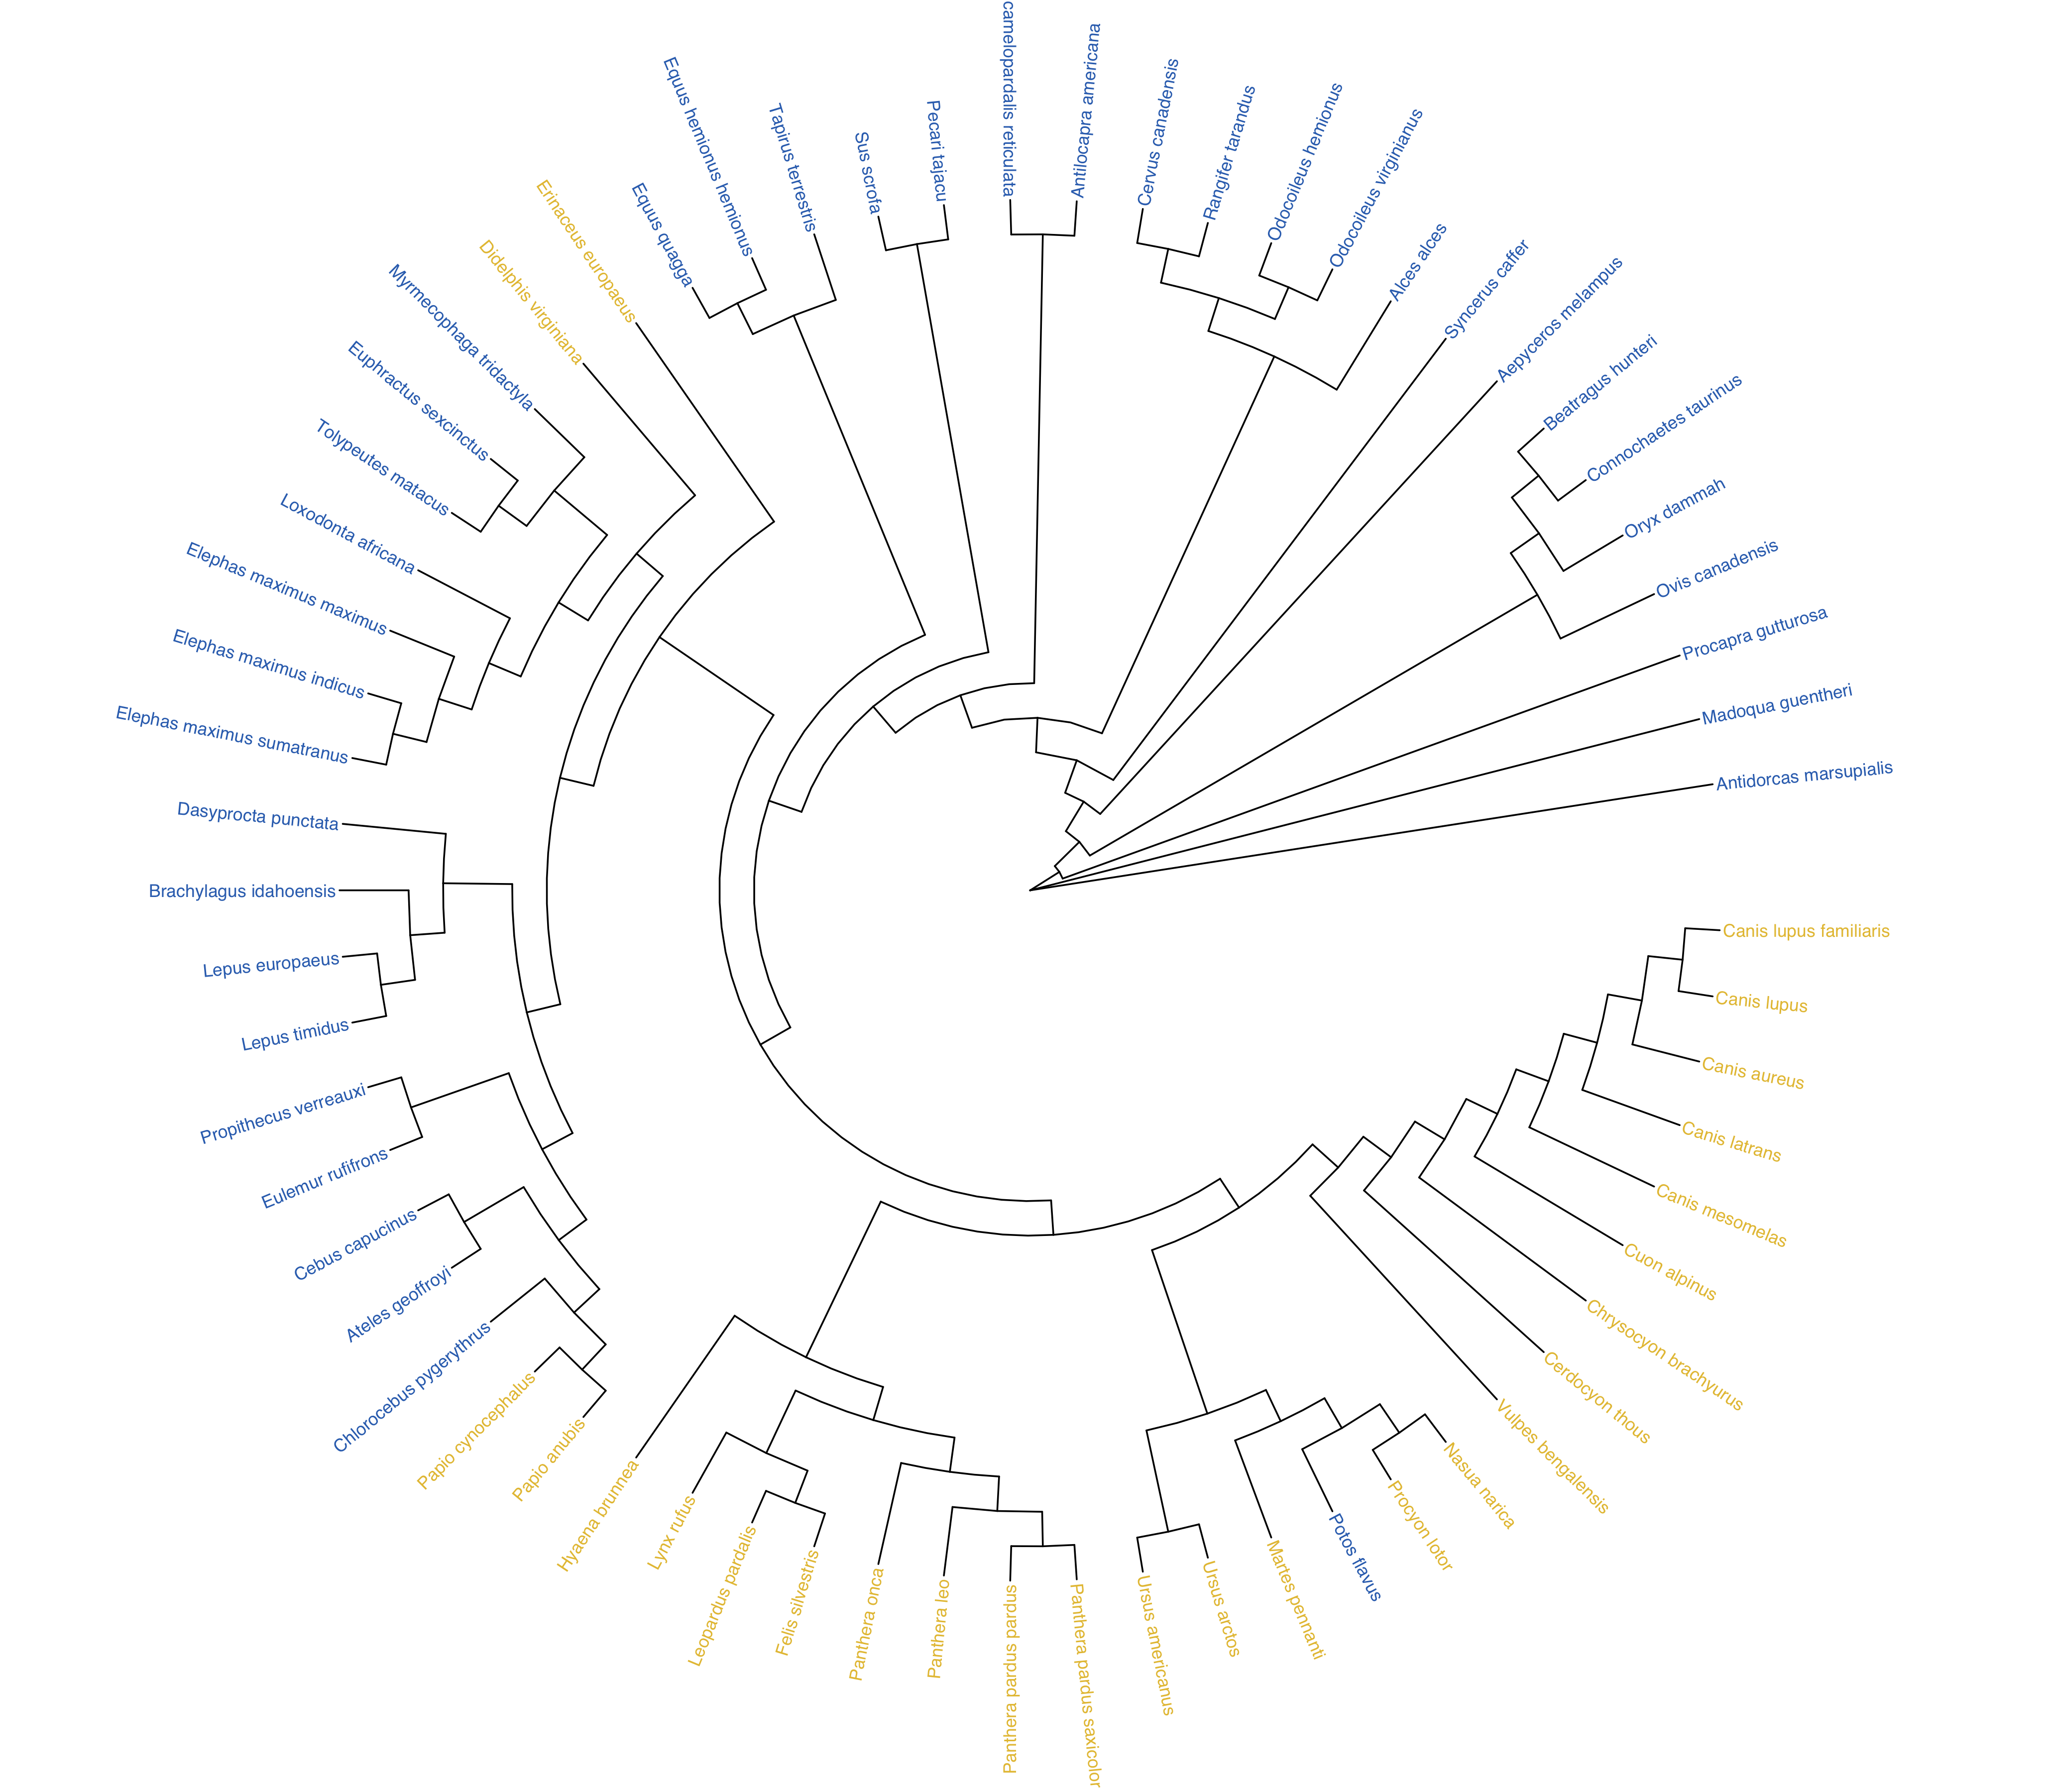
\includegraphics[scale=1]{Phylogeny.png}
\caption{Phylogenetic relationships of the Mammalian species analysed in the main text with species labels coloured by trophic guild (prey in blue, predators in yellow).}
\label{fig:phylogeny}
\end{figure}

%\begin{figure}[!h]
%\centering
%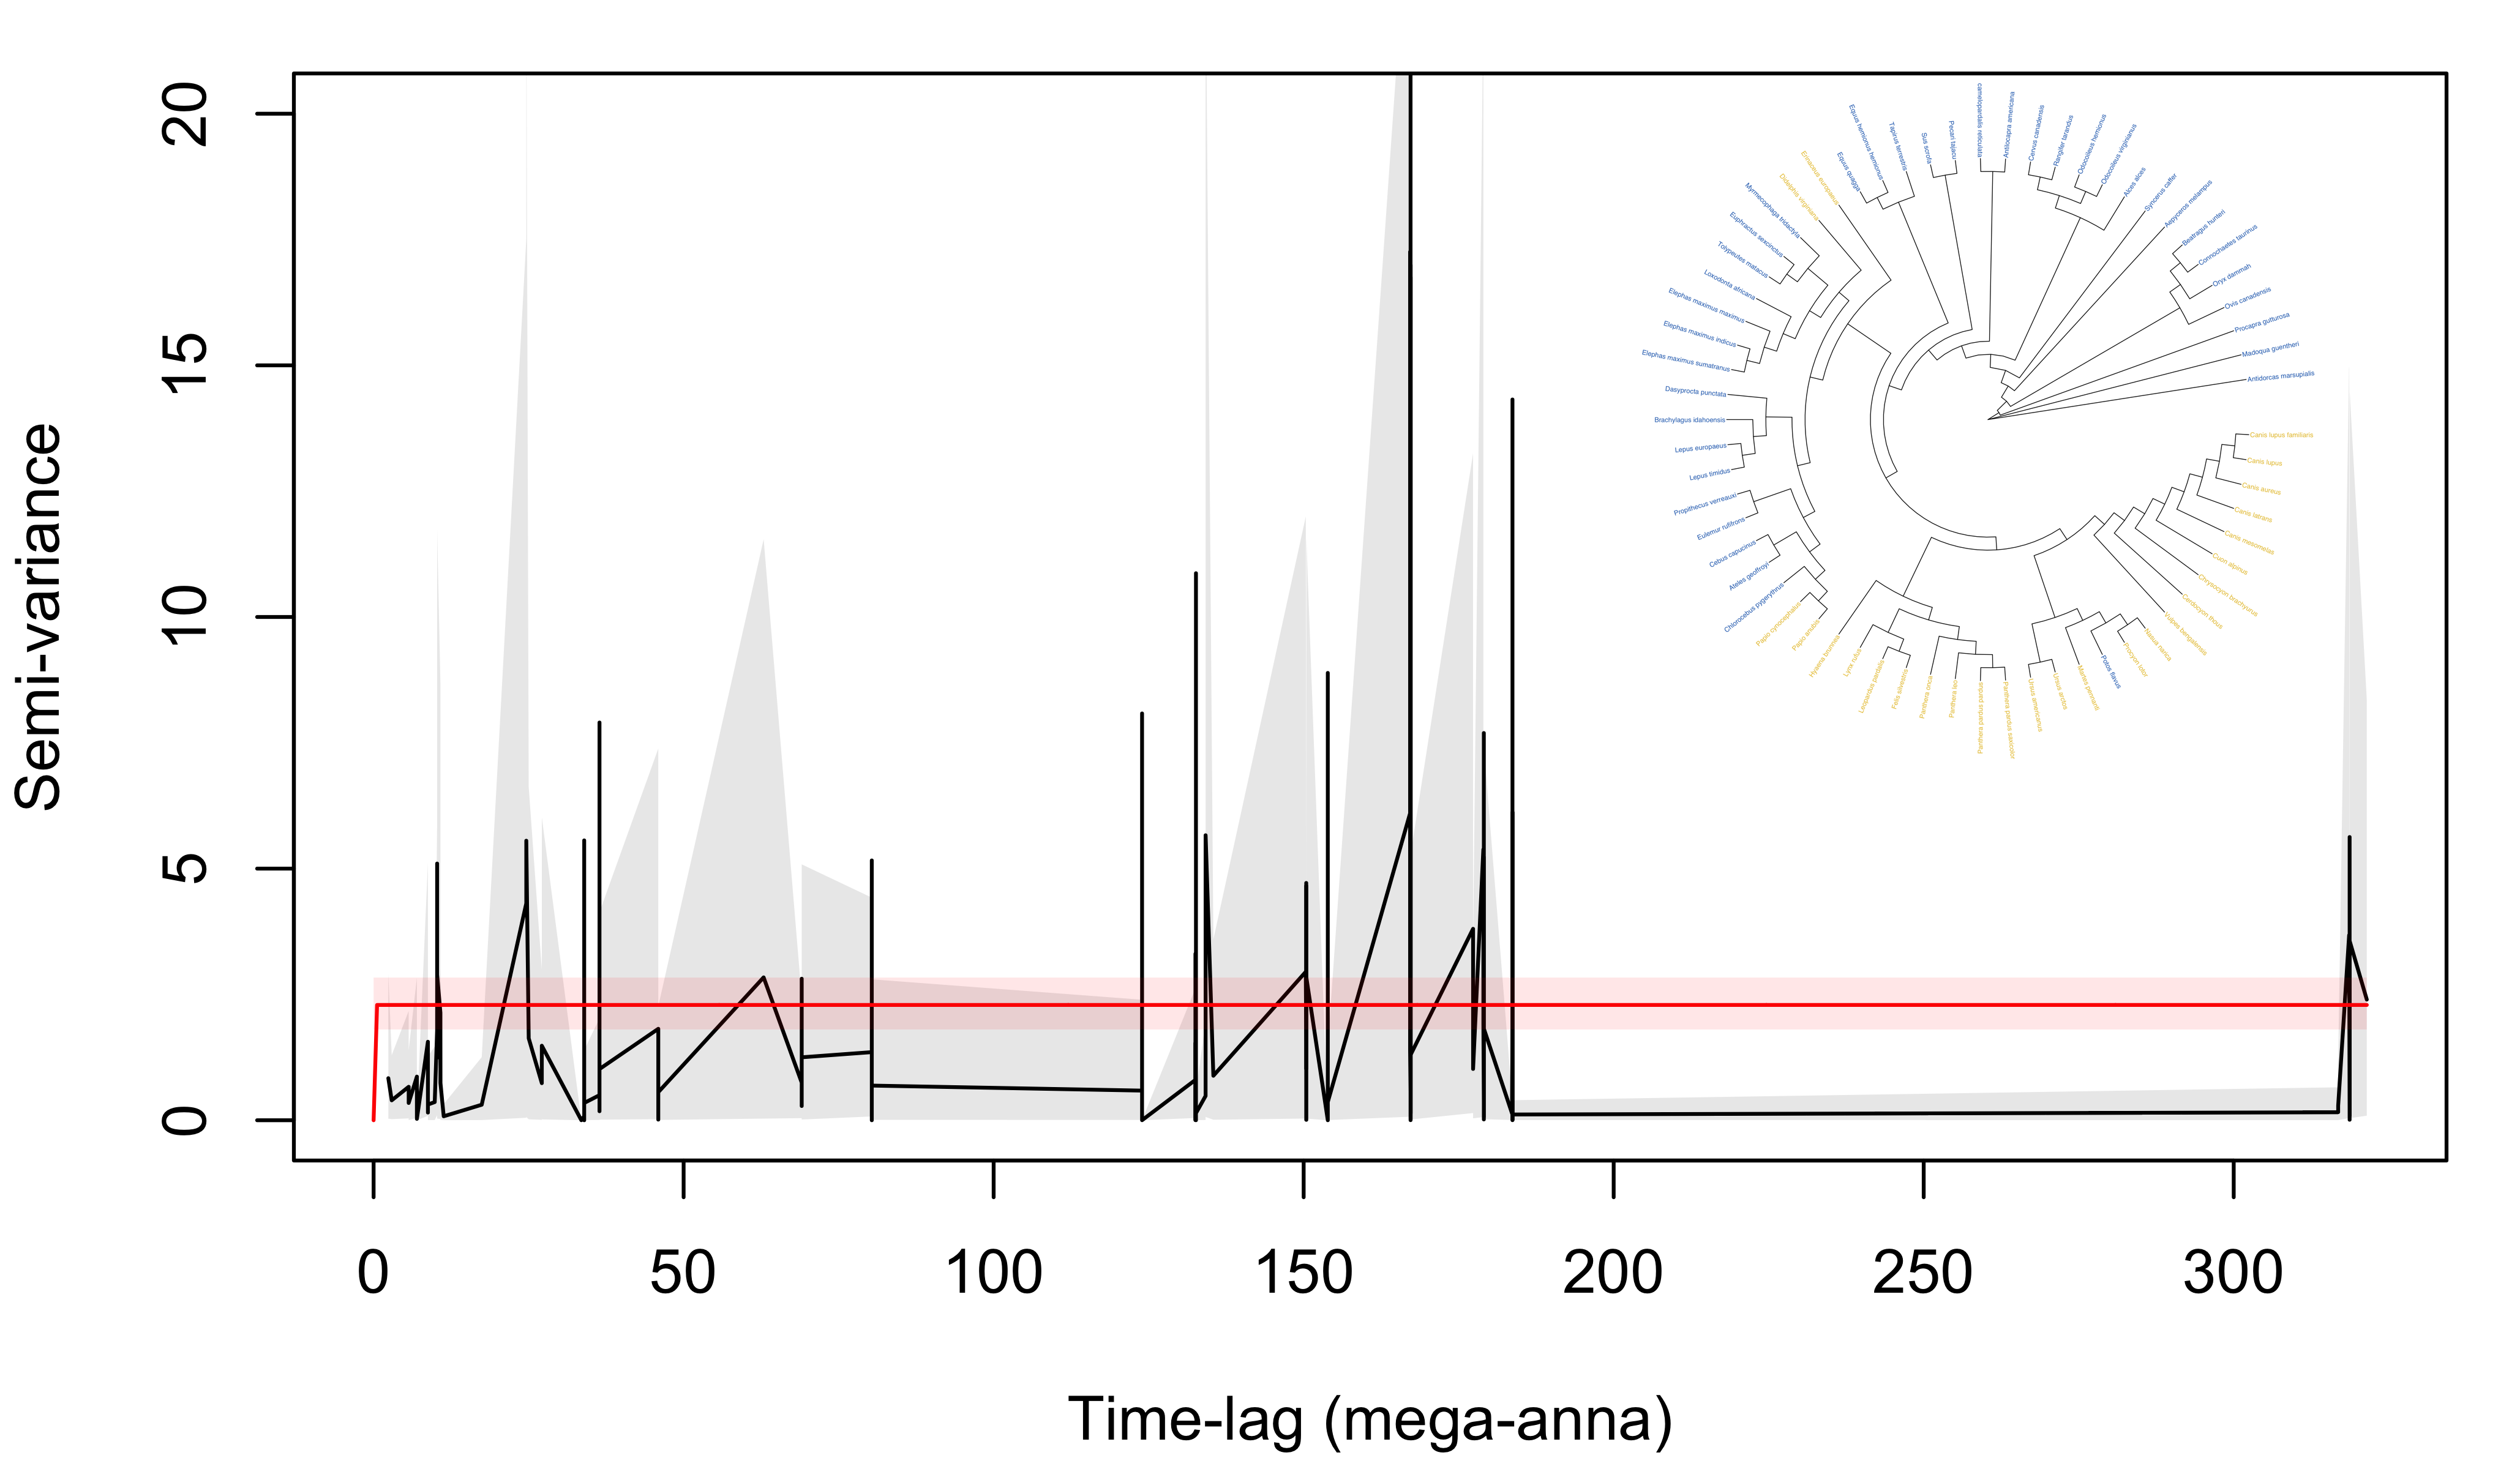
\includegraphics[scale=1]{Ballistic_Motion_SVF.png}
%\caption{Empirical semi-variogram on Mammalian ballistic length scale. The black lines depict the estimated semi-variance at different time lags, wheres the grey shading show the 95\% confidence intervals. The red line and shading depict the estimated semi-variance under an Independent and Identically Distributed IID process. The inset shows the phylogenetic relationships of the Mammalian species analysed in the main text, coloured by trophic group.}
%\label{fig:SVF}
%\end{figure}


The final step in our analyses was to determine whether individual deviations from the allometric relationships in $l_v$ could be described by ecosystem productivity or permeability. We regressed the residuals of the phylogenetically controlled allometric models described above against NDVI and percent forest cover. Models were fitted for predators and prey separately. The relative support for these two models was then assessed by comparing the AICc value of the fitted models against intercept only models.

% the stabilising selection around a mass invariant ration between predator and prey $l_v$ we found in our simulation study could also be observed in the empirical movement data. This required estimating the ratio of predator:prey $l_v$ for each species in our dataset. For this, we used the fitted allometric models described above to predict $l_v$ for the median body mass of each species' predators and prey. We then fit two models to these data, one that included a correlation with body mass, and an intercept only model. The relative support for these two models was then assessed using likelihood ratio tests.


\begin{figure}[!h]
\centering
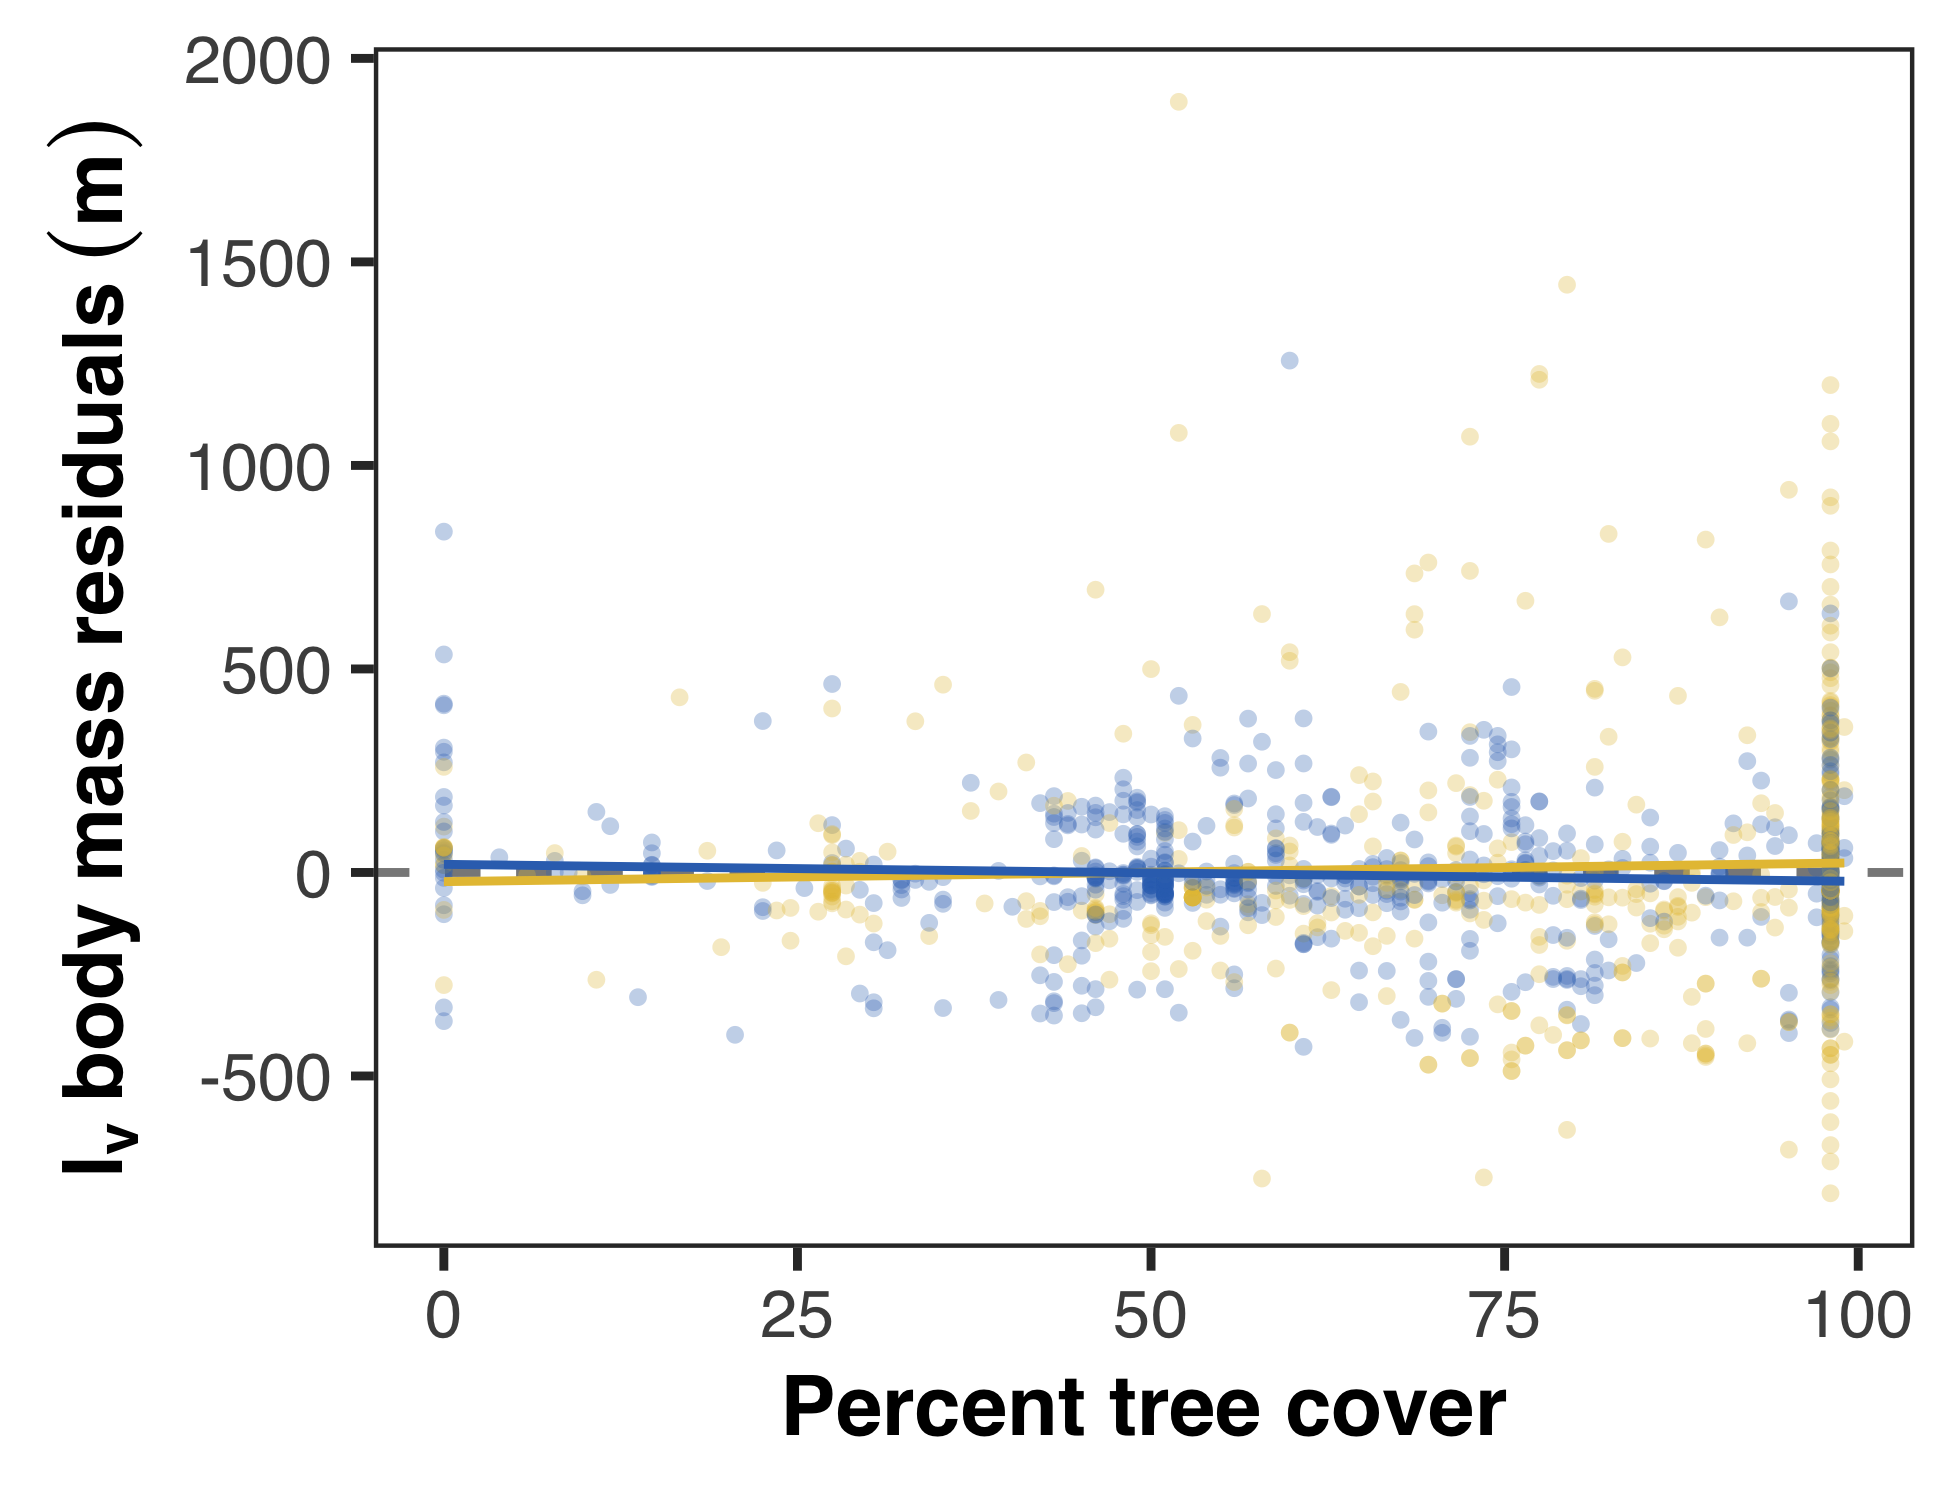
\includegraphics[scale=1]{Empirical_Figure_Trees.png}
\caption{Residuals of the allometric scaling of the ballistic length scale, $l_v$  for prey (blue), as well as predatory (yellow) mammals as a function of the percent tree cover. Each point is an individual ($n=963$) representing 53 species.}
\label{fig:Trees}
\end{figure}

The \texttt{R} scripts used to produce the results presented in this work are openly available on GitHub at \url{https://github.com/NoonanM/BallisticMotion}.


%(SUPPLEMENTARY TABLE WITH MOD SELECTION RESULTS)

\end{document}

